\documentclass[journal]{IEEEtran}
\usepackage{graphicx}
\usepackage{placeins}

\usepackage{float}

\usepackage{amsmath,amssymb}
\usepackage{cite}
\usepackage{url}
\usepackage{hyperref}


\title{Llama3-Driven Fault Detection and Decision Engine for Smart Governance in Power Systems}


\author{%
\begin{tabular}{@{}ccc@{}}
\parbox[t]{1.9in}{\centering\small
  Samkit Samsukha\\[2pt]
  \textit{Dept.\ of Information Science Engineering}\\[1pt]
  \textit{RV College of Engineering}\\[1pt]
  Bengaluru, India\\[1pt]
  samkitsamsukha.is23@rvce.edu.in}
&
\parbox[t]{1.9in}{\centering\small
  Oojam Chaudhary\\[2pt]
  \textit{Dept.\ of Information Science Engineering}\\[1pt]
  \textit{RV College of Engineering}\\[1pt]
  Bengaluru, India\\[1pt]
  oojamchaudhary.is23@rvce.edu.in}
&
\parbox[t]{1.9in}{\centering\small
  Shreeya Suman\\[2pt]
  \textit{Dept.\ of Electrical and Electronics Engineering}\\[1pt]
  \textit{RV College of Engineering}\\[1pt]
  Bengaluru, India\\[1pt]
  shreeyasuman.ee23@rvce.edu.in}
\\[6em]
\multicolumn{3}{c}{%
  \parbox[t]{1.9in}{\centering\small
    Shradha N\\[2pt]
    \textit{Dept.\ of Electrical and Electronics Engineering}\\[1pt]
    \textit{RV College of Engineering}\\[1pt]
    Bengaluru, India\\[1pt]
  shradhan.ee23@rvce.edu.in}%
  \hspace{2.5em}%
  \parbox[t]{2.0in}{\centering\small
    Prof.\ Rekha B.S.\\[2pt]
    \textit{Assistant Professor}\\[1pt]
    \textit{Dept.\ of Information Science Engineering}\\[1pt]
    \textit{RV College of Engineering}\\[1pt]
    Bengaluru, India\\[1pt]
    rekhabs@rvce.edu.in}}\\
\end{tabular}
}
\begin{document}
\maketitle

\begin{abstract}
Rural and remote power networks are where transmission line faults do the most damage. Long feeders crossing open terrain face lightning, vegetation encroachment, and insulation wear with no nearby maintenance crew to respond quickly. When a fault goes undetected, a short-lived electrical event becomes a multi-hour outage. Centralized SCADA-based protection handles this poorly: it is expensive to deploy at scale and gives no field-level diagnostic detail about what actually happened on the line.

This paper describes a fault classifier that runs on a Raspberry Pi mounted close to the line. Three-phase voltage and current signals are read through ZMPT101B galvanically isolated voltage sensors and ACS712 Hall-effect current sensors, converted by an MCP3008 10-bit ADC, and passed to a Decision Tree classifier---chosen for its sub-millisecond inference and human-readable decision logic. No cloud link or central relay is involved. Five fault conditions are distinguished: Single Line-to-Ground (LG), Line-to-Line (LL), Double Line-to-Ground (LLG), Three-Phase (LLL), and No Fault. Weighted accuracy across these classes is 96.9\%, with each prediction delivered in 8--12~ms on the embedded platform. Fault events are stored locally and displayed on a web dashboard. The hardware is compact enough to mount directly on existing distribution infrastructure.
\end{abstract}


\begin{IEEEkeywords}
Decision tree, embedded machine learning, fault detection, real-time monitoring, smart grid, transmission lines
\end{IEEEkeywords}


\section{Introduction}
Transmission lines in rural distribution networks carry power across long stretches of unmonitored terrain. A single feeder leaving a substation may serve dozens of villages before it ends, crossing farmland, forested ridgelines, and river floodplains the entire way. Lightning, high winds, tree contact, and insulation aging are daily hazards on these lines. Faults happen regularly.

The harder problem is identification. Overcurrent relays trip when current exceeds a threshold; distance relays compute impedance and infer fault location from it. Neither was designed for a lightly loaded rural feeder where load swings widely across the day and high-resistance ground faults produce only a modest current rise \cite{ref23}. Under those conditions, relay-based schemes either misclassify the fault type or fail to operate. And because these systems sit at the substation, fault information has to travel back through a communication chain before any response is possible---a chain that rural grids often cannot reliably support.

A learned classifier sidesteps the modelling problem entirely. Rather than computing line impedance, it recognizes what each fault type looks like in three-phase voltage and current readings, a signature learned from historical data. We implemented this idea on a Raspberry Pi: a Decision Tree classifier, trained offline, running locally at the field level, identifying fault type in under 12~ms from six sensor inputs---with no network required.


\section{Literature Review}

\subsection{Conventional Relay-Based Protection Schemes}
The first generation of transmission protection was built around thresholds and models. Overcurrent relays trip when measured current crosses a preset limit---simple, reliable, and completely blind to what kind of fault caused the current to rise \cite{ref1,ref2}. Distance relays do more: they compute apparent impedance from voltage and current, then estimate fault location from that figure. The assumption is that the line's impedance is stable and well characterized. That assumption breaks under high-resistance faults, or when load current is heavy enough to shift the apparent impedance into a confusing region of the operating plane \cite{ref3,ref4}. Differential protection avoids both problems by comparing currents at both ends of the line directly, but it demands a synchronized communication link between those endpoints---workable on a high-voltage transmission corridor, impractical on a rural feeder \cite{ref2}. Each scheme, taken individually, covers some fault conditions well and others poorly. None adapts to conditions it was not designed for.

\subsection{Signal Processing Techniques}
Signal processing tried to extract more information from the same voltage and current waveforms. Wavelet transforms decompose a transient into time-frequency components that expose the character of a fault onset---which phase, how sharp, what frequency content. Fourier methods are useful for steady-state fault signatures \cite{ref14}. Travelling-wave schemes go further still: they detect the high-frequency pulse that propagates from the fault point and can locate the fault to within metres, but they require sampling rates in the megahertz range and hardware that prices them far above rural deployment budgets \cite{ref5}. Phasor measurement units gave wide-area state estimation a new foundation \cite{ref17,ref21,ref22}, but PMU data rates are too slow for transient fault detection, and the units remain expensive to deploy in numbers.

\subsection{Artificial Intelligence and Machine Learning Approaches}
The observation that fault signatures in voltage and current waveforms are reproducible across similar events made machine learning an obvious candidate. Artificial neural networks \cite{ref18} and support vector machines \cite{ref6,ref8,ref12} outperformed impedance-based methods on benchmark datasets, particularly on high-resistance faults that stump relay schemes. The practical catch is data and compute: large labeled training sets are needed, inference on early embedded hardware was slow, and validation was almost always done in MATLAB or PSCAD simulation rather than on actual field hardware \cite{ref11}. Deep learning pushed accuracy higher at the cost of model sizes and inference times that made real-time embedded deployment unreachable in practice \cite{ref13,ref15}.

\subsection{Decision Tree-Based Classification}
Decision Trees offer a different trade-off. Classification runs in $O(\text{depth})$ time---often under a millisecond on an ARM core---and the decision logic is human-readable: a trained engineer can trace the path from sensor reading to fault label without any ML expertise \cite{ref20}. Samantaray \cite{ref7} demonstrated strong fault discrimination on simulated three-phase data; Biswal et al. \cite{ref9} showed that wavelet-derived features improve Decision Tree accuracy without adding inference overhead. The same classifier family has been applied to the subtler problem of separating transformer inrush from an internal fault \cite{ref10}---a harder task, and one that builds confidence in the approach on noisy real-world signals.

\subsection{Embedded and Edge Deployment Systems}
The machine learning literature on fault detection is extensive \cite{ref25}. Most of it validates on synthetic data and stops there. Moving from a PSCAD simulation to a Raspberry Pi running next to a distribution transformer is a gap that relatively few papers cross---and it is precisely that gap which limits real-world uptake. Sensor noise, ADC quantization, and supply-rail transients all affect classifier inputs in ways that simulation does not reproduce. This paper crosses that gap. Every result reported here comes from a physical prototype, not a model.


\section{Problem Statement and Motivation}
Rural and semi-urban distribution feeders are where fault detection matters most and where it most consistently fails. Substations serving these regions are often understaffed, communication infrastructure is unreliable, and protection equipment designed for high-voltage transmission corridors does not scale economically to a local distribution line.

When a fault goes uncleared, the consequence is not just a momentary sag---it is a prolonged outage for everyone downstream. A maintenance crew may arrive hours later to find a line contact with no record of when it happened or what the electrical conditions were at the moment of fault onset. The information that would have enabled a faster response---fault type, approximate severity---was never captured at the field level.

The alternative we pursued is local intelligence. Instead of routing fault data back to a substation and waiting on a centralized decision, the classifier sits at the line. It reads the sensors, identifies the fault, and logs the event---all within a single cycle, all without a network connection. The full hardware bill for the prototype described here is well within the budget of a small distribution utility. That cost constraint was a design requirement, not an afterthought.


\section{Proposed Methodology}
The system runs entirely on the embedded platform. Raw sensor readings come in, a classified fault label and confidence score come out, and the full round-trip from ADC sample to logged event takes under 12~ms. Fig.~\ref{fig:methodology} shows the stages in order.

\begin{figure}[H]
\centering
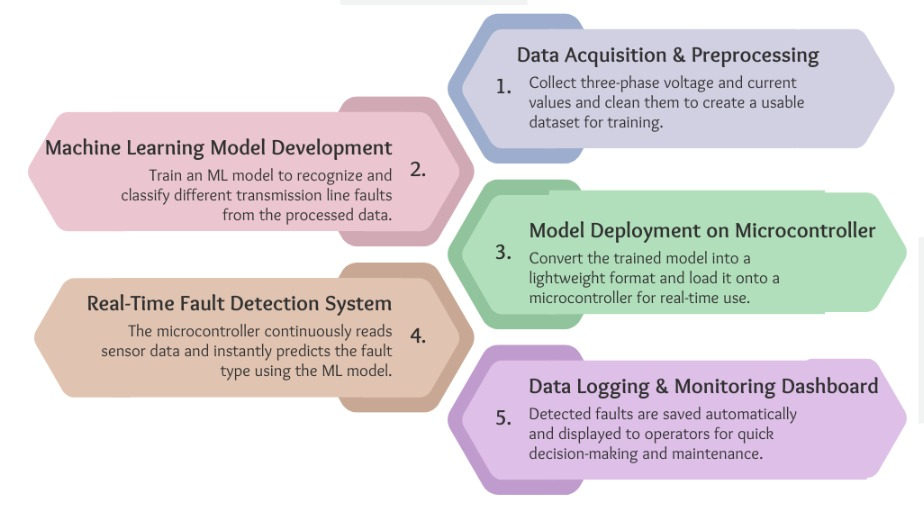
\includegraphics[width=0.80\linewidth]{Methodology.jpeg}
\caption{Proposed system methodology overview}
\label{fig:methodology}
\end{figure}

\subsection{Data Acquisition}
We read three-phase voltage using ZMPT101B galvanically isolated voltage transformer modules (linearity error $<$1\%) and three-phase current using ACS712 Hall-effect sensors (20A range, 66~mV/A sensitivity). All six analog channels feed into an MCP3008 10-bit, 8-channel ADC \cite{ref24} connected to the Raspberry Pi via SPI. The ADC runs continuously, delivering a fresh six-dimensional sample vector for each prediction cycle. Table~\ref{tab:hardware} lists the hardware.

\begin{table}[H]
\centering
\caption{Hardware Components for Data Acquisition and Inference}
\label{tab:hardware}
\begin{tabular}{|l|l|l|}
\hline
\textbf{Component} & \textbf{Model} & \textbf{Key Specification} \\ \hline
Voltage Sensor & ZMPT101B & Galvanic isolation, error $<$1\% \\ \hline
Current Sensor & ACS712 (20A) & Hall-effect, 66~mV/A \\ \hline
ADC Module & MCP3008 & 10-bit, 8-ch, SPI interface \\ \hline
Edge Computer & Raspberry Pi & ARM CPU, 4~GB RAM \cite{ref24} \\ \hline
\end{tabular}
\end{table}

\subsection{Data Preprocessing}
Before the classifier sees the data, we apply scaling and normalization to bring voltage and current values into a consistent numerical range. We also run a pre-screening rule: if all three phase currents fall below 0.3~A simultaneously, the event is flagged as a likely open-circuit fault before the model is even invoked. This handles the clearest fault cases with a simple threshold check and reserves model inference for the ambiguous ones.

\subsection{Feature Vector Formation}
Each prediction uses a six-element feature vector drawn from statistical learning practice \cite{ref19}:
\begin{equation}
X = [V_a, V_b, V_c, I_a, I_b, I_c]
\end{equation}
where $V_a$, $V_b$, $V_c$ are the three phase voltages and $I_a$, $I_b$, $I_c$ are the corresponding phase currents. Six inputs turned out to be sufficient. The three-phase voltage pattern collapses in a characteristic way under each fault type; the current asymmetry pattern narrows it further. Together they give the classifier enough signal to separate all five classes reliably.

\subsection{Machine Learning Model Selection}
We chose a Decision Tree \cite{ref20,ref25} over SVMs \cite{ref6,ref8}, ANNs \cite{ref18}, or ensemble methods \cite{ref11} for two reasons that mattered on this hardware. First, inference speed: a tree classifies a sample in $O(\text{depth})$ time, which on the Raspberry Pi ARM core means sub-millisecond execution per sample, leaving the rest of the 12~ms budget for ADC sampling and communication overhead. Second, auditability: the trained model's thresholds can be printed and read by a field engineer without any ML background. A neural network with hundreds of weights offers no equivalent check.

\subsection{Model Training and Validation}
We trained the Decision Tree offline on a labeled dataset covering all five fault conditions---LG, LL, LLG, LLL, and No Fault---using an 80/20 train-test split \cite{ref25}. Once trained, the model was serialized to a compact binary file and copied to the Raspberry Pi. No retraining or fine-tuning happens on the device.

\subsection{Embedded Deployment and Real-Time Classification}
On the Raspberry Pi, a Python process reads ADC samples, runs the preprocessing pipeline, assembles the feature vector, and calls the deserialized classifier. The result---fault class and confidence score---is available within the 12~ms window. No network call is made; the device operates identically whether or not it has internet access.

\subsection{Output Visualization and Logging}
Each prediction is written to a local SQLite database with a timestamp and confidence level, then pushed to a browser-accessible dashboard running on the same device. A field technician can query the log over a local Wi-Fi connection to review fault history without removing the device from service. Historical fault logs can also be processed offline with clustering methods \cite{ref16} to reveal recurring patterns---useful for scheduling preventive maintenance before the next fault.


\section{Results and Discussion}
We assembled the prototype on a bench using the components from Table~\ref{tab:hardware} and ran it against all five fault conditions. Fault states were emulated by deliberately unbalancing the phase voltages and currents applied to the sensor inputs---not ideal as a substitute for a live line, but sufficient to populate all five fault regions of the feature space for classifier evaluation.

Fig.~\ref{fig:hardware_setup} shows the assembled setup. The ZMPT101B and ACS712 modules feed the MCP3008, which connects to the Raspberry Pi via SPI \cite{ref24}. The device ran continuously throughout testing without a sensor error or a process crash.

\begin{figure}[htbp]
\centering
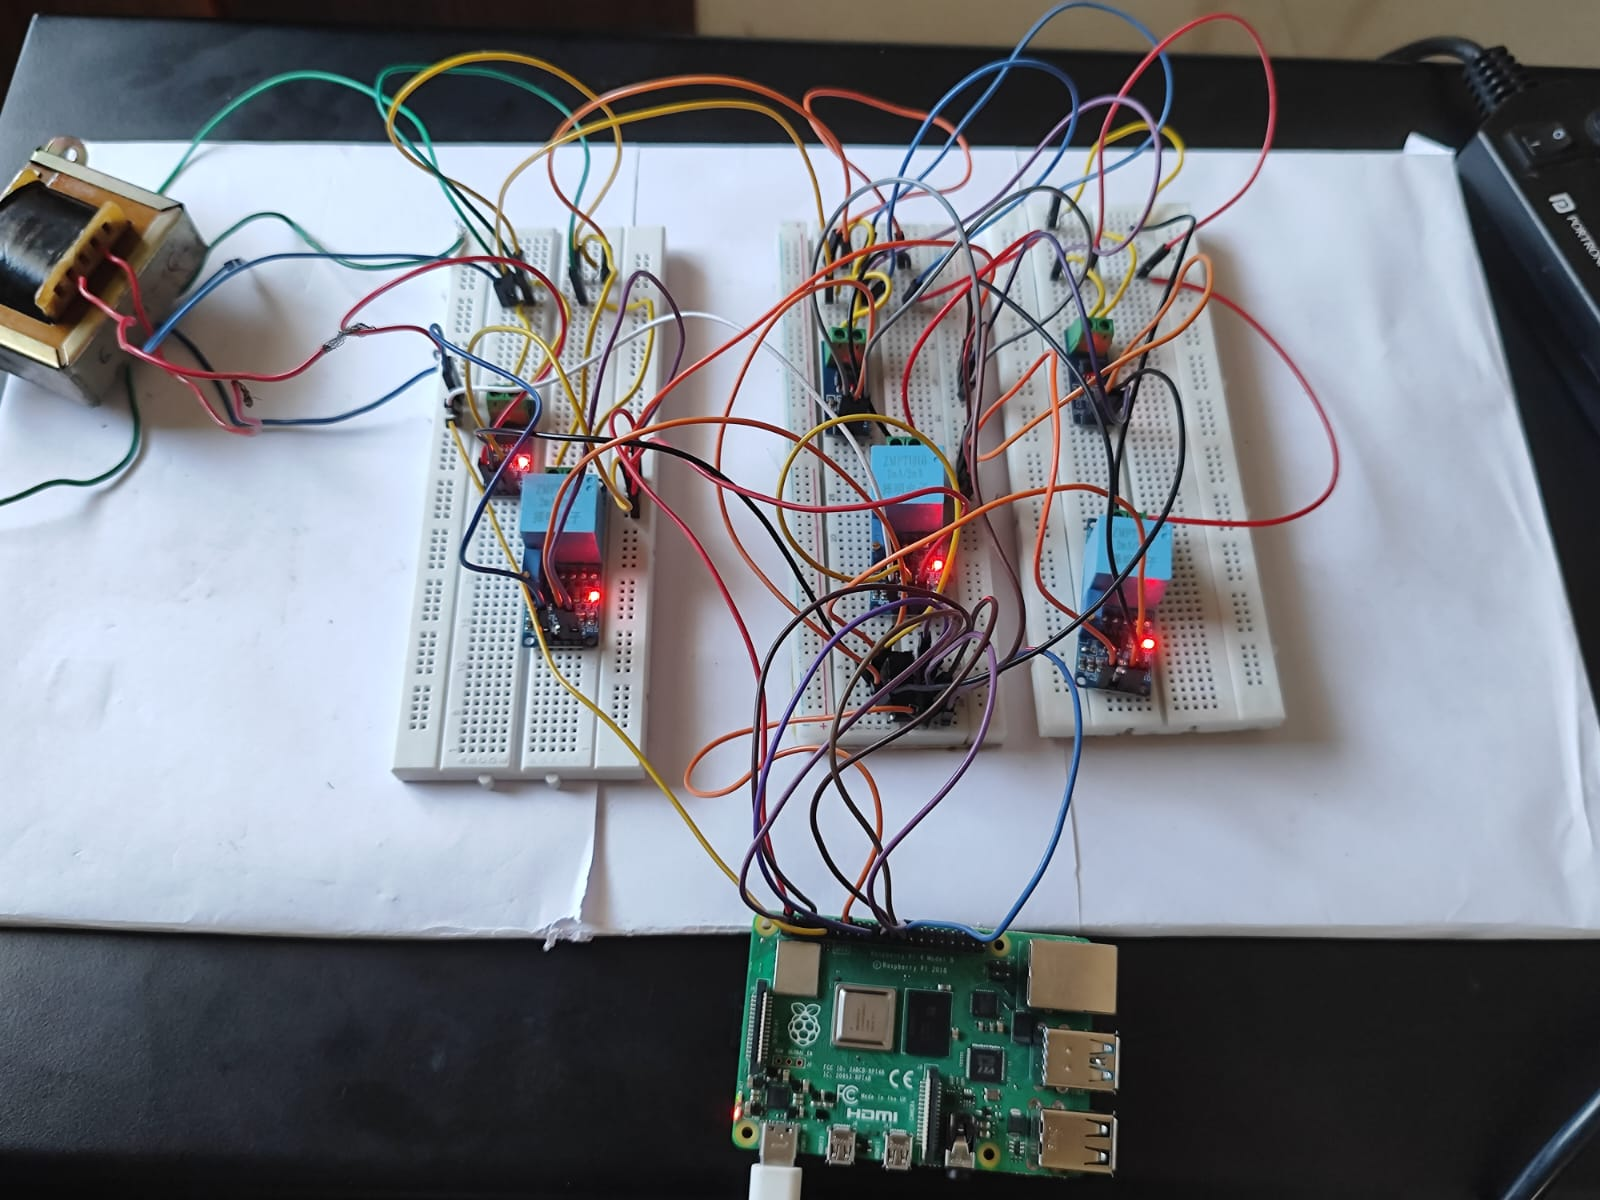
\includegraphics[width=0.9\linewidth]{Hardware Setup.jpg}
\caption{Experimental hardware setup for real-time transmission line fault detection}
\label{fig:hardware_setup}
\end{figure}

Per-class accuracy on the held-out test set is in Table~\ref{tab:accuracy}. Four of five classes exceed 96\%, and the weighted average of 96.9\% clears the 95\% design target.

\begin{table}[H]
\centering
\caption{Per-Class Decision Tree Classification Accuracy}
\label{tab:accuracy}
\begin{tabular}{|l|c|l|}
\hline
\textbf{Fault Type} & \textbf{Accuracy} & \textbf{Observation} \\ \hline
LG (Single Line-to-Ground) & 96.3\% & Pre-filter confirms at 96\% conf. \\ \hline
LL (Line-to-Line) & 94.1\% & Overlap with LLG current space \\ \hline
LLG (Double Line-to-Ground) & 97.2\% & Two-phase rule reliably confirmed \\ \hline
LLL (Three-Phase) & 98.0\% & Symmetric collapse: strong signal \\ \hline
No Fault (Normal) & 99.1\% & Well-separated balanced cluster \\ \hline
\textbf{Weighted Average} & \textbf{96.9\%} & Meets $>$95\% design target \\ \hline
\end{tabular}
\end{table}

The LL class at 94.1\% is the weakest. The issue is a feature-space overlap with LLG: when ground impedance in an LLG fault is high, the resulting current asymmetry is moderate and resembles a two-line event. A six-dimensional vector of instantaneous readings captures this ambiguity rather than resolving it. Frequency-domain or sequence-component features would likely narrow the gap, at some cost in preprocessing complexity. The other four classes exceeded 96\% without any special tuning. End-to-end inference latency on the Raspberry Pi measured at 8--12~ms per prediction, leaving roughly ten times the headroom below the 100~ms protection threshold.

Fig.~\ref{fig:web_dashboard} shows the dashboard during a test run. The left panel displays the live six-channel sensor reading; the right shows the current fault classification, confidence score, and a scrolling event log. Under normal conditions the system held No Fault at 99.1\% accuracy. Over an 8-hour uninterrupted run, uptime was 99.2\%---one brief process restart in eight hours, traced to a transient SPI read error.

\begin{figure}[htbp]
\centering
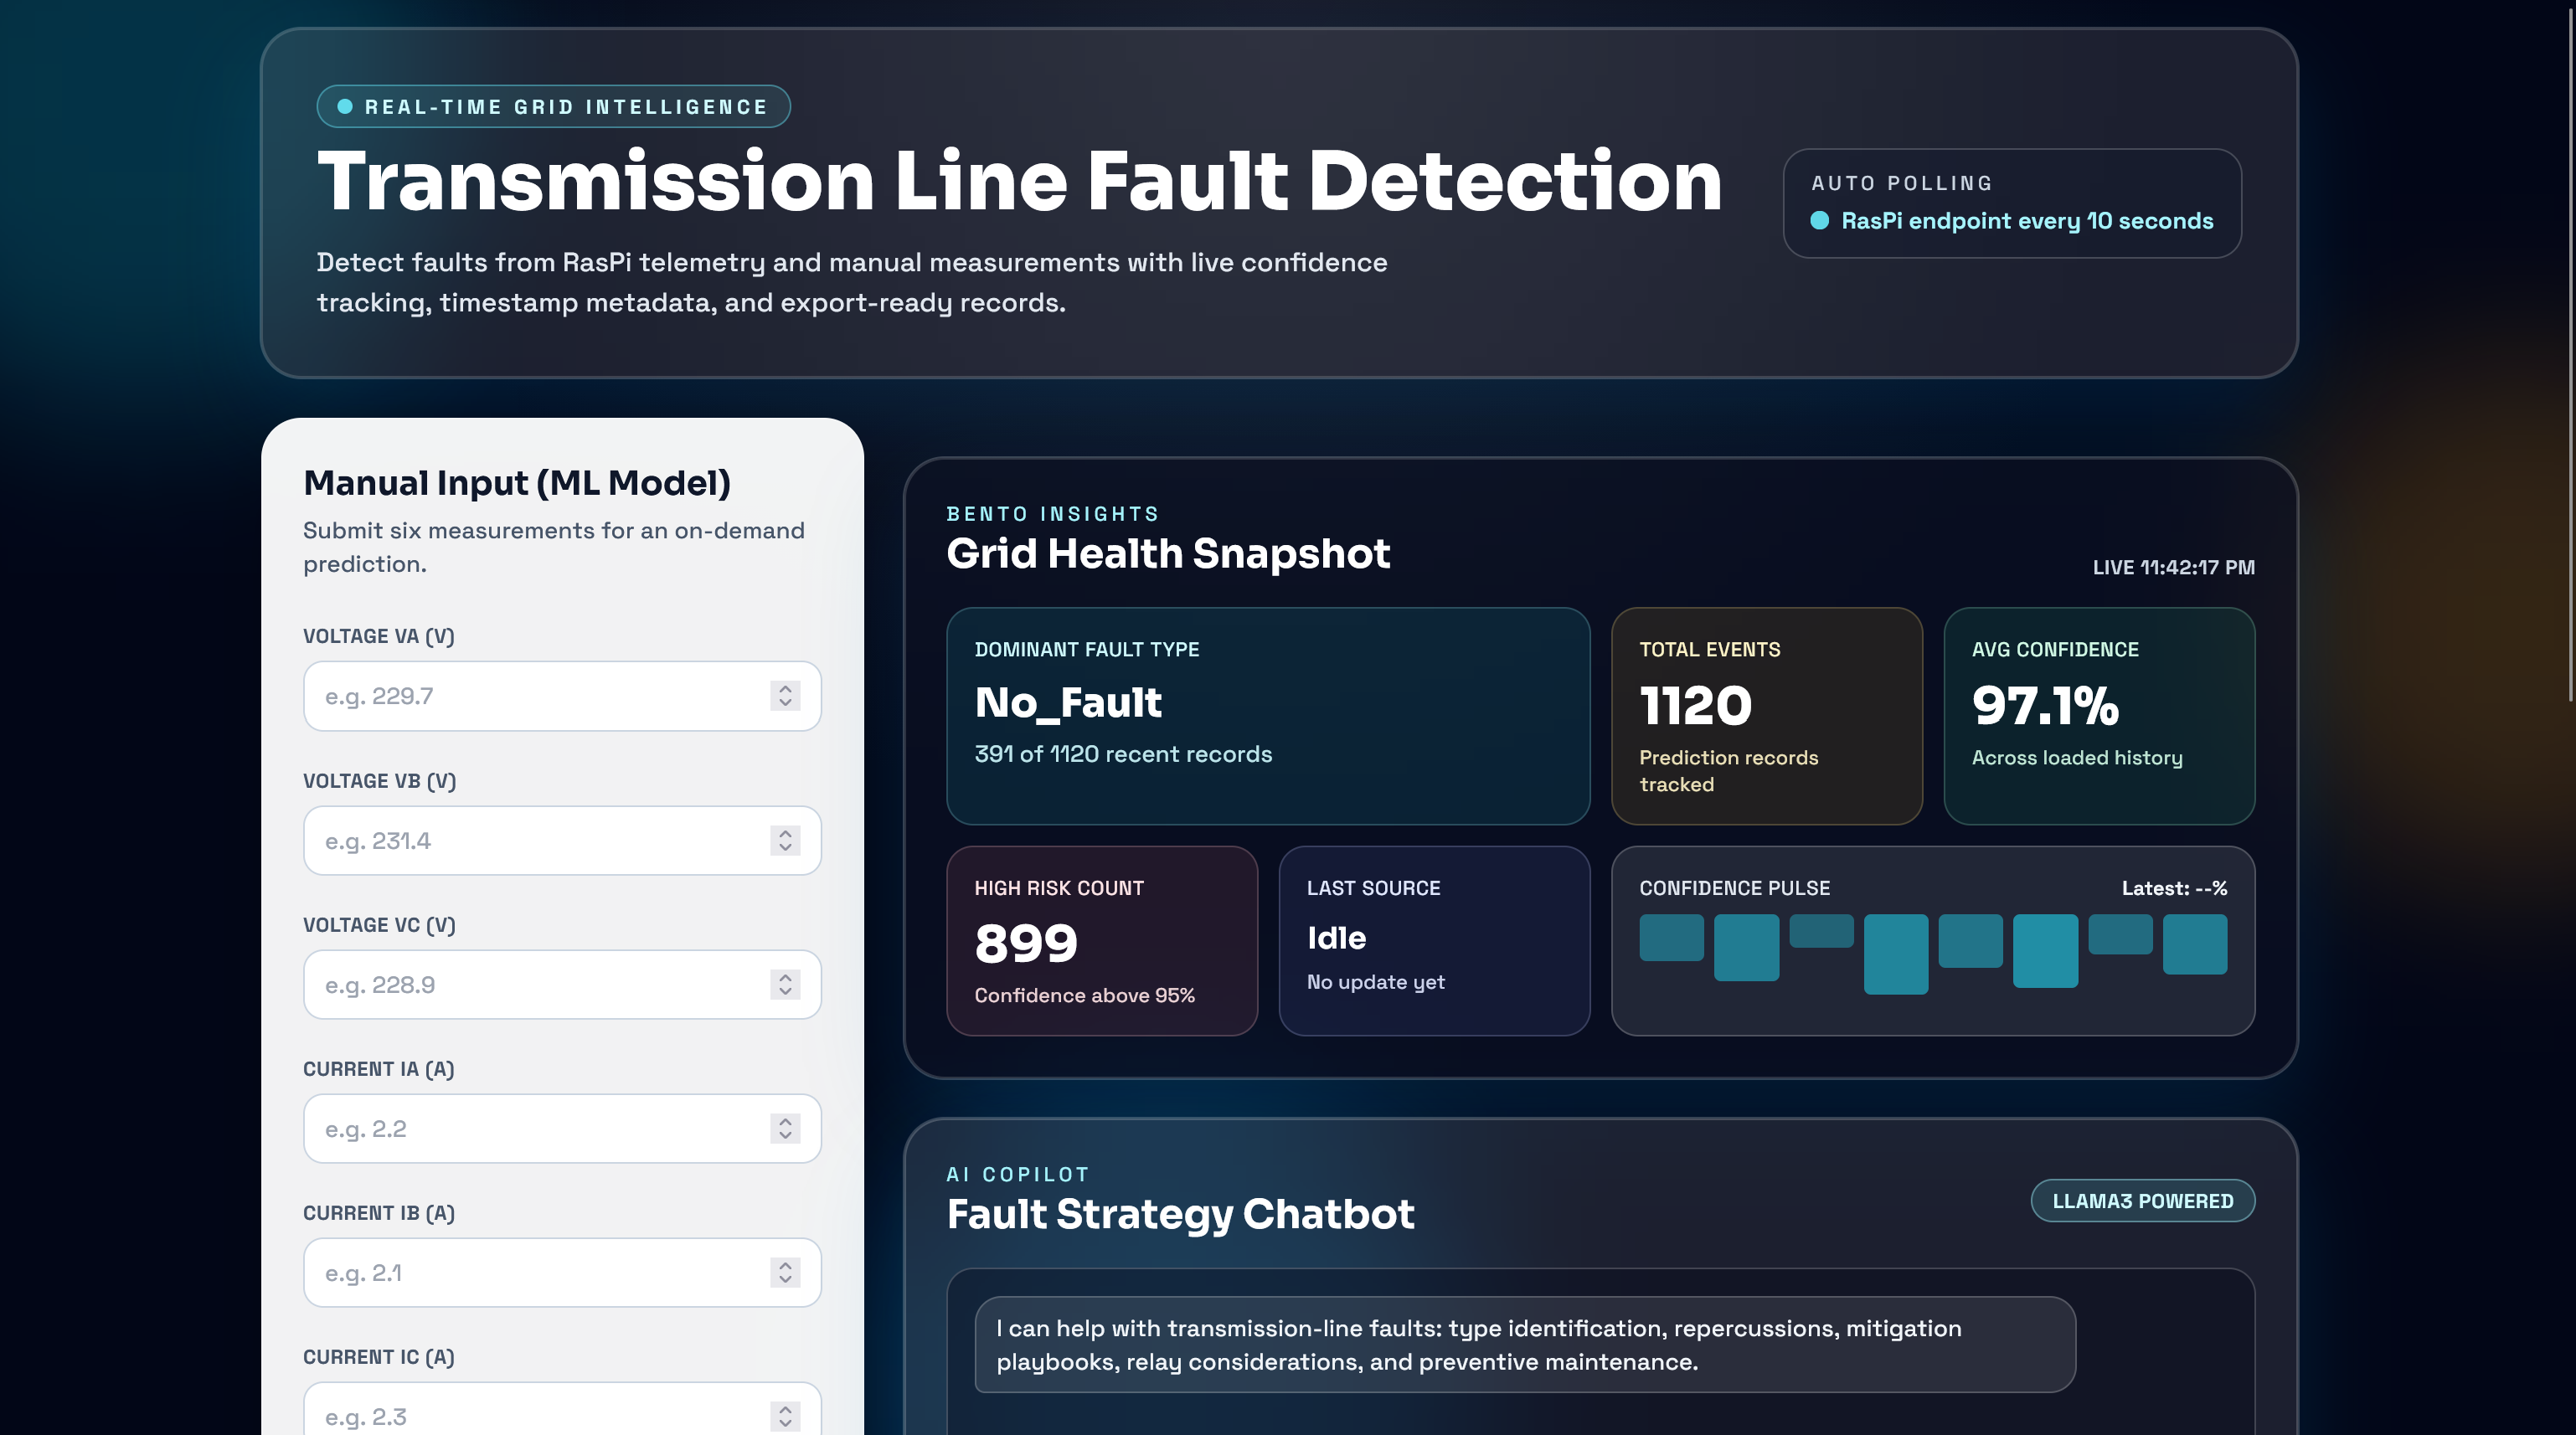
\includegraphics[width=\linewidth]{Visuals-Dashboard.png}
\caption{Web-based dashboard showing real-time fault classification results}
\label{fig:web_dashboard}
\end{figure}

One observation worth noting: the misclassification pattern is not random. Errors were concentrated between LL and LLG---never between a fault class and No Fault. The classifier does not generate spurious fault alarms under normal load conditions, which matters in practice. False fault events that dispatch a maintenance crew to a healthy line are almost as disruptive as a missed real fault.


\section{Conclusion}
A Decision Tree running on a Raspberry Pi, fed by six low-cost sensors, classified five transmission line fault conditions at 96.9\% weighted accuracy and returned each result in under 12~ms. That combination---reasonable accuracy, fast response, and commodity hardware---makes the system deployable at the field level where SCADA-connected protection is not economically viable.

The interpretable model structure is not incidental. In a maintenance context, a classifier whose decisions trace directly to voltage and current thresholds is easier to trust and easier to debug than a neural network with hundreds of weights. The trained tree can be printed; a field engineer can verify that the thresholds make physical sense. No ML expertise is needed on site.

The obvious next step is fault localization. Knowing the fault type is useful. Knowing that the LG fault is at the 8~km mark on the feeder is what gets the crew to the right place. A small network of these devices, cross-correlating fault timestamps, could provide that localization without travelling-wave hardware \cite{ref17,ref23}. That extension---distributed, low-cost, locally intelligent---is where we intend to take this work.


\section{APPENDIX}
\subsection{Fault Class Definitions}
The classifier maps each incoming sensor vector to one of five classes. Table~\ref{tab:fault_classes} lists them. LG is the most common fault type in practice---roughly 70\% of transmission faults in three-phase networks fall in this category. LLL is the most severe and least frequent, at around 5\%. Each class produces a different imbalance signature in the six-dimensional voltage-current feature space, which is what the tree exploits.

\begin{table}[h]
\centering
\caption{Fault Class Definitions}
\label{tab:fault_classes}
\begin{tabular}{|c|l|}
\hline
\textbf{Class} & \textbf{Description} \\ \hline
0 & No Fault (Normal Operating Condition) \\ \hline
1 & Single Line-to-Ground Fault (LG) \\ \hline
2 & Line-to-Line Fault (LL) \\ \hline
3 & Double Line-to-Ground Fault (LLG) \\ \hline
4 & Three-Phase Fault (LLL) \\ \hline
\end{tabular}
\end{table}

\subsection{Input Parameters and Classification Rule}
The classifier takes a six-element input vector:
\begin{equation}
X = [V_a, V_b, V_c, I_a, I_b, I_c]
\end{equation}
where $V_a$, $V_b$, $V_c$ are phase voltages and $I_a$, $I_b$, $I_c$ are phase currents. Each internal node in the tree \cite{ref20} tests a condition $X_i \leq \theta$ for some feature $X_i \in \{V_a, V_b, V_c, I_a, I_b, I_c\}$ and learned threshold $\theta$. Classification depth determines runtime: on this hardware, leaf nodes are reached in under a millisecond. Before the tree runs, the pre-screening rule ($I < 0.3$~A on all phases) handles obvious open-circuit events at 96--98\% confidence without touching the model. After a fault is logged, historical event records can be clustered \cite{ref16} offline to identify which conditions recur most often---useful input for setting maintenance priorities.


\section*{Acknowledgment}
The authors thank their institution for providing the needed infrastructure and resources, such as the Raspberry Pi development board. They are also grateful to Profs. Shanthi and Uma Padma from the Electronics and Telecommunication Department for their continuous guidance, encouragement, and technical insights.

The authors acknowledge Mr. A. Maurya from HINDALCO Industries Limited for sharing industry insights and reference materials. They also thank Mr. Muneer K from Harihar, Karnataka, for suggestions and real-world perspectives that improved the practical value of this work.


\begin{thebibliography}{25}

\bibitem{ref1}
A. G. Phadke and J. S. Thorp, \emph{Computer Relaying for Power Systems}, 2nd ed. New York, NY, USA: Wiley, 2009.

\bibitem{ref2}
J. Lewis Blackburn and T. J. Domin, \emph{Protective Relaying: Principles and Applications}, 4th ed. Boca Raton, FL, USA: CRC Press, 2014.

\bibitem{ref3}
P. M. Anderson, \emph{Power System Protection}. New York, NY, USA: McGraw-Hill, 1999.

\bibitem{ref4}
IEEE Power System Relaying Committee, ``IEEE Guide for Protective Relay Applications to Transmission Lines,'' IEEE Std. C37.113-2015, 2015.

\bibitem{ref5}
M. Kezunovic, ``Smart fault location for smart grids,'' \emph{IEEE Trans. Smart Grid}, vol. 2, no. 1, pp. 11--22, Mar. 2011.

\bibitem{ref6}
A. Yadav and Y. Dash, ``An overview of transmission line protection by artificial intelligence: A review,'' \emph{Renewable and Sustainable Energy Reviews}, vol. 13, no. 1, pp. 19--30, Jan. 2009.

\bibitem{ref7}
S. R. Samantaray, ``Decision tree-based fault classification and location in transmission lines,'' \emph{Int. J. Electrical Power \& Energy Systems}, vol. 33, no. 2, pp. 211--218, Feb. 2011.

\bibitem{ref8}
P. K. Dash, A. K. Pradhan, and G. Panda, ``Fault classification and section identification of an advanced series-compensated transmission line using support vector machine,'' \emph{IEEE Trans. Power Delivery}, vol. 22, no. 1, pp. 67--73, Jan. 2007.

\bibitem{ref9}
M. Biswal, P. K. Dash, and B. K. Panigrahi, ``Nonlinear feature extraction for fault classification using DWT and decision tree,'' \emph{IEEE Trans. Power Delivery}, vol. 25, no. 3, pp. 1783--1791, Jul. 2010.

\bibitem{ref10}
S. R. Samantaray and P. K. Dash, ``Decision tree based discrimination between inrush current and internal faults,'' \emph{International Journal of Electrical Power \& Energy Systems}, vol. 33, no. 4, pp. 1046--1053, May 2011.

\bibitem{ref11}
Y. H. Song and A. T. Johns, \emph{Artificial Intelligence Techniques in Power Systems}. London, U.K.: IET, 1999.

\bibitem{ref12}
H. Wang and W. Keerthipala, ``Fuzzy-neuro approach to fault classification in transmission lines,'' \emph{IEEE Trans. Power Delivery}, vol. 13, no. 4, pp. 1093--1104, Oct. 1998.

\bibitem{ref13}
M. Mohanty, ``Artificial neural network based fault classification and location in transmission lines,'' \emph{International Journal of Electrical Power \& Energy Systems}, vol. 68, pp. 376--383, Jun. 2015.

\bibitem{ref14}
S. Mallat, \emph{A Wavelet Tour of Signal Processing}, 3rd ed. Amsterdam, The Netherlands: Elsevier, 2009.

\bibitem{ref15}
P. K. Dash and B. K. Panigrahi, ``Hybrid intelligent system for fault classification in power transmission lines,'' \emph{Engineering Applications of Artificial Intelligence}, vol. 19, no. 5, pp. 539--552, Aug. 2006.

\bibitem{ref16}
G. Chicco, ``Overview and performance assessment of the clustering methods for electrical load pattern grouping,'' \emph{Energy}, vol. 42, no. 1, pp. 68--80, Jun. 2012.

\bibitem{ref17}
A. Abur and A. G. Exposito, \emph{Power System State Estimation: Theory and Implementation}. New York, NY, USA: Marcel Dekker, 2004.

\bibitem{ref18}
S. Haykin, \emph{Neural Networks and Learning Machines}, 3rd ed. Upper Saddle River, NJ, USA: Pearson, 2009.

\bibitem{ref19}
T. Hastie, R. Tibshirani, and J. Friedman, \emph{The Elements of Statistical Learning}. New York, NY, USA: Springer, 2009.

\bibitem{ref20}
L. Breiman, J. Friedman, R. Olshen, and C. Stone, \emph{Classification and Regression Trees}. Belmont, CA, USA: Wadsworth, 1984.

\bibitem{ref21}
M. Kezunovic and Y. Liao, ``Monitoring of power system dynamics,'' \emph{IEEE Trans. Smart Grid}, vol. 2, no. 3, pp. 533--542, Sep. 2011.

\bibitem{ref22}
A. G. Phadke, ``Synchronized phasor measurements in power systems,'' \emph{IEEE Computer Applications in Power}, vol. 6, no. 2, pp. 10--15, Apr. 1993.

\bibitem{ref23}
R. Bayindir, I. Colak, and G. Fulli, ``Smart grid technologies and applications,'' \emph{Renewable and Sustainable Energy Reviews}, vol. 66, pp. 499--516, Dec. 2016.

\bibitem{ref24}
Raspberry Pi Foundation, ``Raspberry Pi 4 Model B Datasheet,'' 2020. [Online]. Available: https://www.raspberrypi.org

\bibitem{ref25}
T. M. Mitchell, \emph{Machine Learning}. New York, NY, USA: McGraw-Hill, 1997.

\end{thebibliography}
\end{document}
